\section[1978年高考数学试卷及答案(全国卷)理科]{1978年普通高等学校招生考试(全国卷)\\\Huge{理科数学}}
\begin{questions}
	\question
	\begin{parts}
		\part 分解因式:$x^2 - 4xy + 4y^2 - 4z^2$.

			\begin{solution}
				\begin{align*}
					 & = (x-2y)^2 - 4z^2    \\
					 & = (x-2y+2z)(x-2y-2z)
				\end{align*}
			\end{solution}

		\part 已知正方形的边长为$a$,求侧面积等于这个正方形的面积,高等于这个正方形边长的直圆柱体的体积.

			\begin{solution}
				设直圆柱体的直径为$r$,则有侧面积:
				\begin{equation*}
					S_侧 = 2\pi{r}a
				\end{equation*}
				因为直圆柱体的侧面积等于正方形的面积,因此有:
				\begin{align*}
					2\pi{r}a = a^2 \\
					r = \frac{a}{2\pi}
				\end{align*}
				所以可得直圆柱体的体积为:
				\begin{align*}
					V & = \pi{r^2}a               \\
					  & = \pi \frac{a^2}{4\pi^2}a \\
					  & = \frac{a^3}{4\pi}
				\end{align*}
			\end{solution}

		\part 求函数$y=\sqrt{\lg(2+x)}$的定义域.

			\begin{solution}
				\begin{cenum}
					\item 由$\lg(2+x) \geqslant 0$得:
					      \begin{align*}
						      2+x \geqslant 1 \\
						      x \geqslant -1
					      \end{align*}

					      \begin{center}
						      \begin{tikzpicture}
							      \begin{axis}[
									      xmin = -4, xmax = 4,
									      ticks=both
								      ]
								      \addplot[domain=-3:3, blue!70, thick]{log10(x+2)};
								      \addlegendentry{$\lg(x+2)$}
							      \end{axis}
						      \end{tikzpicture}
					      \end{center}

					\item 由$2+x > 0$得:
					      \begin{equation*}
						      x > -2
					      \end{equation*}
					\item 综上,函数的定义域为$\{x|x\geqslant-1\}$.

				\end{cenum}
			\end{solution}

		\part 不查表求$\cos\ang{80}\cos\ang{35} + \cos\ang{10}\cos\ang{55}$的值.
			\begin{solution}
				\begin{align*}
					 & = \cos\ang{80}\cos\ang{35} + \sin\ang{80}\sin\ang{35} \\
					 & = \cos(\ang{80} - \ang{35})                           \\
					 & = \cos\ang{45}                                        \\
					 & = \frac{\sqrt{2}}{2}
				\end{align*}
			\end{solution}
		\part 化简: $\displaystyle\left( \frac14 \right)^{-\frac12}\cdot
				\frac{(\sqrt{4ab^{-1}})^3}{(0.1)^{-2}(a^3b^{-4})^{\frac12}}$.
			\begin{solution}
				\begin{align*}
					 & = 2 \cdot \frac{(4ab^{-1})^{\frac32}}{100a^\frac32b^{-2}}                 \\
					 & = 2 \cdot \frac{4^{\frac32}a^{\frac32}b^{-\frac32}}{100a^{\frac32}b^{-2}} \\
					 & = 2 \cdot \frac{8\sqrt{b}}{100}                                           \\
					 & = \frac4{25}\sqrt{b}
				\end{align*}
			\end{solution}
	\end{parts}

	\question 已知方程$kx^2 + y^2 =
		4$,其中$k$为实数,对于不同范围的$k$值,分别指出方程所代表图形的类型,并画出显示其数量特征的草图.

	\begin{solution}
		\begin{penum}
			\item $k = 0$时,$y=\pm2$,这是两条平行于$x$轴的直线;
			      \begin{center}
				      \begin{tikzpicture}
					      \begin{axis}[xmin=-3, xmax=3, ymax=3, ymin=-3]
						      \addplot[domain=-2:2, green!50!blue, thick]{2};
						      \addplot[domain=-2:2, red!50!blue, thick]{-2};
						      \addlegendentry{$y=2$}
						      \addlegendentry{$y=-2$}
						      \node[below left] at (0,2) {$2$};
						      \node[below left] at (0,-2) {$-2$};
					      \end{axis}
				      \end{tikzpicture}
			      \end{center}

			\item $k > 0$时,图形是半轴分别为$\frac{2}{\sqrt{k}}$和$2$的椭圆,其中当$k = 1$时,长短轴相等形状为圆形;
			\item $k < 0$时,图形是双曲线.
			      \begin{center}
				      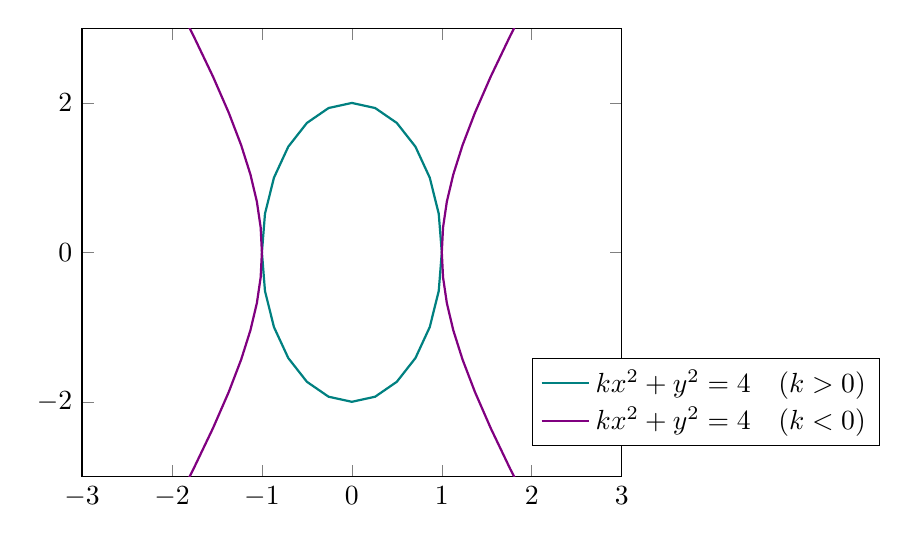
\begin{tikzpicture}
					      \begin{axis}[xmin=-3, xmax=3, ymax=3, ymin=-3,
							      legend style={at={(axis cs:2,-2)}, anchor=west}]
						      \addplot[domain=0:360, green!50!blue, thick]({cos(x)}, {2*sin(x)});
						      \addlegendentry{$kx^2 + y^2 = 4 \quad(k>0)$}
						      \addlegendentry{$kx^2 + y^2 = 4 \quad(k<0)$}
						      \addplot[domain=-2:2, red!50!blue, thick]({cosh(x)}, {2*sinh(x)});
						      \addplot[domain=-2:2, red!50!blue, thick]({-cosh(x)}, {2*sinh(x)});
					      \end{axis}
				      \end{tikzpicture}
			      \end{center}
		\end{penum}
	\end{solution}

	\question 如图,$AB$是半圆的直径,$C$是半圆上的一点,直线$MN$切半圆于$C$点,$AM\perp MN$于$M$点,$CD\perp
		MN$于$N$点,$CD\perp AB$于$D$点,求证:
	\begin{penum}
		\item $CD=CM=CN$;
		\item $CD^2=AM\cdot BN$.
	\end{penum}
	\begin{center}
		\begin{tikzpicture}[scale=1.5]
			\def\pangle{55}
			\coordinate(o) at (0,0);
			\coordinate(c) at (\pangle:1);
			\coordinate(a) at (-1,0);
			\coordinate(b) at (1,0);
			\coordinate(d) at ($(a)!(c)!(b)$);
			\coordinate(t) at ({1/cos(\pangle)}, 0);
			\coordinate(m) at ($(c)!(a)!(t)$);
			\coordinate(n) at ($(c)!(b)!(t)$);
			\draw (a) arc [start angle=180, end angle=0, radius=1];
			\draw (a) -- (b) (c) -- (d) (a) -- (m) -- (n) -- (b);
			\draw (m)node[above]{$M$} (c) node[above]{$C$} (n) node[above]{$N$} (a)node[below left]{$A$} (d)node[below]{$D$}
			(b)node[below right]{$B$};

		\end{tikzpicture}
	\end{center}

	\begin{proofsolution}
		\begin{center}
			\begin{tikzpicture}[scale=1.5]
				\def\pangle{55}
				\coordinate(o) at (0,0);
				\coordinate(c) at (\pangle:1);
				\coordinate(a) at (-1,0);
				\coordinate(b) at (1,0);
				\coordinate(d) at ($(a)!(c)!(b)$);
				\coordinate(t) at ({1/cos(\pangle)}, 0);
				\coordinate(m) at ($(c)!(a)!(t)$);
				\coordinate(n) at ($(c)!(b)!(t)$);
				\draw (a) arc [start angle=180, end angle=0, radius=1];
				\draw (a) -- (b) (c) -- (d) (a) -- (m) -- (n) -- (b);
				\draw (m)node[above]{$M$} (c) node[above]{$C$} (n) node[above]{$N$} (a)node[below left]{$A$} (d)node[below]{$D$}
				(b)node[below right]{$B$} (o) node[below]{$O$};
				\draw[dashed, blue] (o) -- (c) -- (a) (b) -- (c);

				\draw[angle radius=10pt, red] pic[draw]{right angle=n--m--a} pic[draw]{right angle=n--c--o} pic[draw]{right
						angle=m--n--b};

			\end{tikzpicture}
		\end{center}
		\begin{penum}
			\item
			      \begin{cenum}
				      \item 连接圆心$O$与$C$点.
				            \begin{align*}
					             & \because AM \perp MN \land BN \perp MN  \land OC \perp MN \\
					             & \therefore AM \parallel BN \parallel OC                   \\
					             & \because AO = BO                                          \\
					             & \therefore MC = CN
				            \end{align*}
				      \item	连接$AC$.
				            \begin{align*}
					             & \because AO = OC                                            \\
					             & \therefore \angle{OAC} = \angle{OCA}                        \\
					             & \because AM \parallel CO                                    \\
					             & \therefore \angle{MAC} = \angle{ACO}                        \\
					             & \therefore \angle{DAC} = \angle{MAC}                        \\
					             & \because \angle{AMC} = \angle{ADC} = \ang{90} \land AC = AC \\
					             & \therefore \triangle{ACM} \cong \triangle{ACD}              \\
					             & \therefore MC = CD                                          \\
					             & \therefore MC = CN = CD
				            \end{align*}
			      \end{cenum}
			\item 连接$BC$.
			      \begin{align*}
				       & \because \angle{CDB} = \angle{CNB} = \ang{90} \land CD = CN \land CB = CB                   \\
				       & \therefore \triangle{BDC} \cong \triangle{BNC}                                              \\
				       & \therefore BD = BN                                                                          \\
				       & \because \angle{BCD} = \angle{CAB} = \angle{CAM} \land \angle{AMC} = \angle{CDB} = \ang{90} \\
				       & \therefore \triangle{AMC} \sim \triangle{CDB}                                               \\
				       & \therefore \frac{AM}{MC} = \frac{CD}{DB}                                                    \\
				       & \therefore \frac{AM}{CD} = \frac{CD}{BN}                                                    \\
				       & \therefore CD^2 = AM\cdot BN
			      \end{align*}
		\end{penum}
	\end{proofsolution}

\end{questions}
